% !BIB TS-program = biber

\documentclass[a4paper,11pt]{article}
%-----------------------------------------------------------
\usepackage{amsmath}
\usepackage{blindtext}
\usepackage{graphicx}
\usepackage{enumitem}
\usepackage{listings}
\usepackage{hyperref}
\usepackage[font={small},labelfont=bf]{caption}
\usepackage[margin=1cm]{caption}
\usepackage[backend=biber]{biblatex}
\addbibresource{reference.bib}

%-----------------------------------------------------------
%-----------------------------------------------------------
\begin{document}
%-----------------------------------------------------------
\begin{titlepage}
	\centering
	
\includegraphics[width=0.15\textwidth]{img/photo.jpg}\par\vspace{1cm}
	{\scshape\LARGE The University of Auckland \par}
	\vspace{1cm}
	{\scshape\Large COMPSCI 780\par}
	\vspace{1.5cm}
	{\huge\bfseries Benchmarking software obfuscators An experimental approach\par}
	\vspace{2cm}
	{\Large\itshape Rafik Nasraoui\par}
	\vfill
	supervised by\par
	Dr.~Clark \textsc{Thomborson}

	\vfill

% Bottom of the page
	{\large \today\par}
\end{titlepage}
%-----------------------------------------------------------
\begin{abstract}
\textit{
	The optimisation of software code execution speed is a key consideration in any software project.
	A high level of security, to the extent that all ‘hacks’ are rendered impossible, is also of crucial importance to most software. One way of protecting sensitive information is through obfuscation, which aims to make the computer programme unintelligible to a human being, without altering the core functionality of the programme. 
	A problem with obfuscation, is that it may slow down the processing speed of a software, and therefore reduce the overall user experience.
	We analyse the results of a preliminary experiment that benchmarks the execution time of a fixed-width boolean circuit, where the width of the circuit is increased with each execution. The circuit represents an approximation of a result of a functional encryption operator, i.e. of an obfuscation. The experiment collects cache data generated by the executing system’s hardware performance counters, to measure the execution time of the circuit.
}
\end{abstract}

\section{Introduction}
Security and data privacy are critical aspects of most software programmes. The
need for such security can derive from the need for compliance with government
regulations, and individual and company privacy requirements. The protection of
sensitive information and industry data is also vital for software to stay
competitive. The ability of ‘hackers’ to extract sensitive data is continuously
advancing, and so software data protection must also continuously evolve, in
order to keep ahead of such efforts.
\par
One of the mechanisms that could be implemented in the future to protect data is
obfuscation. Software obfuscation aims at making computer programs unintelligible
for a human being, without affecting the functionality of the software. Although
software must be delivered into the hands of the public in order for the public
to make use of the software, obfuscation hides the information contained within
the software, including the code itself, by rendering it illegible to a user or
hacker.
\par
Obfuscation has potential useful applications in preventing reverse engineering
and thereby protecting Intellectual Property, and in enabling secure software
distribution. Obfuscation can also be a powerful means of encrypting data.
\par
Until recently, there was no formal definition of obfuscation, and all techniques,
including manually obscuring data, could be given the label “obfuscation”. These
techniques do not have quantifiable security and anyone with a debugger, a compiler
a day's worth of effort can reverse engineer code that has been obfucated with the
current best efforts\cite{Hsieh}.
\par
Recent developments in cryptography theory have however produced a formal definition of
obfuscation, which will most assuredly lead to an increased interest in the field,
in the hope that obfuscation can be practically applied to protect software in the
near future. The theory also suggests that the adversray work factor, \.i.e. the
work required to be performed by an adversary to break the obsucation, scales exponentially
with the program runtime.\cite{Hsieh}
\par
However, the drawback of using obfuscation is that it may be ultimately limited
by the hardware on which the software is run. Obfuscators need to produce obfuscated
programs using available computing resources in a commercially relevant amount of
time. These obfuscations then need to be evaluated by end users in relatively
similar, if not more challenging conditions, in terms of hardware performance
and functionality. Normal encryption methods in general have small variable size
and a low number of instructions, and therefore require little run time to execute.
Obfuscators however are technically challenging to implement, and the number of
variables and instructions arising from an obfuscation may surpass the limits of
the hardware within which the software is run.
\par
This paper aims to test the hypothesis that obfuscation is limited by the hardware
it runs on. Should this hypothesis prove true, it would place serious constraints
on the practicality of obfuscation in most situations.

\section{Background}
This section outlines the definitons of boolean circuits and indistinguishability obfuscation that are essential to this paper.
\par
\subsection{Boolean Circuits}
Real world programs are compiled into a sequence of machine instructions that can be interpreted by a processing unit (CPU) manipulating a finite number of $bits$ at a time. The CPU is a chip that is made of logical gates that are made of a few transistors. In this context, boolean circuits are a powerful model that can express any algorithm we can run on a CPU\cite{cpu}.
\par
Complexity Theory defines a \textit{Boolean Circuit} $C$ with $n$ inputs and $m$ outputs as a finite, labeled, directed acyclic graph. It contains $n$ nodes with no incoming edges or ancestors; called the input nodes and $m$ nodes with no outgoing edges or successors, called the output nodes. All other nodes are called gates and represent the logic operation AND, OR and NOT\cite{bool}. Simply put, a \textit{Boolean Circuit}  is a diagram showing a combination of logic operators to a drive an output from an input. By associating a boolean function with each gate, a boolean circuit computes an arbitrary function $f \in F :  \{0,1\}^n \to \{0,1\}^m$. Two common properties are associated with boolean circuits: 
\begin{enumerate}  
	\item The $size$ of a circuit is the number of non-input vertices that it contains. 
	\item The $depth$ of a circuit is the length of the longest directed path from an input vertex to an output vertex. 
\end{enumerate}
Because of the acyclic and oriented nature of the circuit, each node can be represented as receiving its inputs from a lower order depth only. To evaluate a circuit, we process the nodes in an increasing order of depth by applying the associated boolean operation on the input vertices. The result is passed to the higher order nodes.
\par
\begin{figure}[h]
	\center
	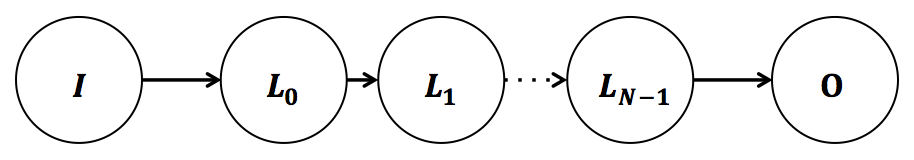
\includegraphics[width=0.9\textwidth]{img/graph.png}
	\caption{Simple high level representation of a boolean circuit}
\end{figure}
\par
Size and Depth give an indication of the computation necessary to evaluate a circuit. Size is a rough measure of the computation time a single processor would need for a sequential circuit evaluation. Depth is an important cost metric for time efficiency in a parallel execution environment where the size is no longer the main bottleneck\cite{notes}. 
\par 
Another  established circuit property that is relevant to our study is the $width$ of a circuit\cite{clark}. If the circuit is arranged in levels such that the input of each level are connected from lower order levels exclusively, we define the width $w$ as the maximum number of gates contained in single level.
\par
The formal study of circuit complexity is beyond the scope of this paper. We should however quickly mention the notion of \textit{Circuit Family}. Our definition limits the size of input to a fixed number of bits. The notion of boolean circuit $C_n$ computing $f_n$  is generalised to a family of circuits C which is a collection of boolean circuits $\{C_1, C_2, C_3, \cdots\}$ such that there is one circuit $C_i$ that computes F on i inputs.
%-----------------------------------------------------------
%
%
%-----------------------------------------------------------
\subsection{Indistinguishability Obfuscation}
Obfuscation must meet two requirements, as defined by Barak et al.\cite{barak}:
\begin{enumerate}
	\item The functionality of the obfuscated programme must remain identical to the functionality of the original, un-obfuscated programme.
	\item Anything (and everything) that can be efficiently computed from Oc can be efficiently computed given oracle access to C. i.e. Oc does not disclose any information about the input other than what C does. 
\end{enumerate}
The first requirement is trivial and means that for any input programme $C$, an Obfuscator $O$ produces a new programme $O_C$ where the functionality of $O_C$  is identical to the functionality of $C$. This condition means that given an input space $I$ we have $ \forall x \in I, C(x) = O_C(x)$.
\par
The second requirement is less trivial and also known as the Virtual Black Box $(VBB)$ requirement. It implies that there is no ``leakage`` of information, other than the input and the output. This means that it is impossible to tell whether an output was produced from the computation of $C$, or from the computation of $O_C$. An adversary can learn a predicate of $O_C(x)$ with the same probability of learning it from $C(x)$. 
\par
Barak et al. concluded that the VBB requirement is impossible to attain in certain situations\cite{barak}, however, it is possible to come close to meeting the second requirement, which in practice is enough to maintain the usefulness of obfuscation as an effective security measure. This is done by modifying the requirement of VBB, and replacing it with two weaker definitions that can still result in rendering a programme unintelligible in a meaningful and practical way. These definitions are namely indistinguishability $iO$ and differing-input obfuscation $diO$, which require that for any circuit pair $C_1$ and $C_2$ from the same circuit family $C$ that compute the same functionality $f$, the obfuscated versions of $C_1$ and $C_2$; $iO(C_1)$ and $iO(C_2)$ are perfectly indistinguishable. The probability of an observer being able to tell if an output was generated from $iO(C_1)$ or from $iO(C_2)$ is negligible.
\par
Some work has been done within the scientific community to develop real-life obfuscations that meet the requirements given by Barak et al. Garg et al.\cite{garg} published an obfuscation construction valid for all polynomial-size, log-depth circuits constructed under novel algebraic hardness assumptions. Based on this work, Banescu et al.\cite{tum} published a proof-of-concept implementation of this $iO$ construction.
However, to date there is no efficient practical implementation of Barak et al.\cite{barak} indistinguishability obfuscation requirement. 
This lack of ready-made obfuscators does not limit the ability of this paper to prove or disprove the hypothesis that obfuscation is limited by the hardware restraints of the operating system, as a simulation of an obfuscation-like process is sufficient for this purpose.


\section{Methodology}
We now describe the algorithm used to simulated an obfuscated boolean circuit and the tools used to measure its evaluation impact on a hardware platform.
\subsection{BPW Generation} 
Thomborson proposed a space-efficient and computationally-appropriate file format (BPW) for the evaluation of very large Boolean functions with bounded program widths\cite{clark}. Gates of a circuit are represented by descriptors holding information about their type (AND, OR, $\dots$) and are sequentially encoded inside the file's body. In our experiment we generate random boolean circuits (which evaluates a random boolean function) with varying width $w = \{ 10^3, 10^4, 10^5, 10^6, 10^7, 10^8\}$ for a fixed circuit size $N = 10^8$. The relationship between a circuit width and depth is $ N = w \times D $, so for $ w = N$ the circuit has depth 1.
\par
The generated circuits are represented using a simplified BPW format by storing the gate type and the input indices only and by making some assumptions about the properties of the circuit under test. In particular, we make the following assumptions about the size of the circuit's inputs and outputs as well as the manner outputs from level $L_i$ are passed to gates in level $L_{i+1}$ as inputs.
\begin{enumerate}  
\item All circuits have size $N = 10^8$
\item A circuit input array has size $w$.
\item Any given level $L$ has exactly $w$ gates.
\item Every gate has only one output.
\item A circuit output array has size $w$.
\item Any given gate from a level $L_i$ has between one and three inputs that come from level $L_{i-1}$ exclusively, such that:\break $G_i = f(X)$, where $f$ is a boolean operator and $X$ is an 8-byte array of size 1, 2 or 3. 
\item The output of a gate is written inside the output array at the same index of the gate. $G_i(X) = Output$ $array[i]$.
\end{enumerate}
The \textit{rand()} method from the \textit{C} standard library was used to attribute a random type to a gate, as well as assign its input indices.

\subsection{Evaluation}
A circuit evaluation is sequential at both gate and layer level. During execution, gates of a level $L_i$ are processed in ascending order of index in the level. Inputs indices for a gate are randomly distributed over [0, $w$-1]. Every gate retrieves its relevant inputs as described by the gate descriptor. Once a gate is processed, its output is stored in the output array at the same index as the gate. Once all the gates of level $L_i$ are processed, the execution cursor moves to level $L_{i+1}$. The random distribution of gate input indices will significantly affect the overall performance of the circuit for large $w$, as the entire input array cannot fit in the cache. Figure \ref{fig:level} describes how a level is evaluated.
\begin{figure}[h]
	\center
	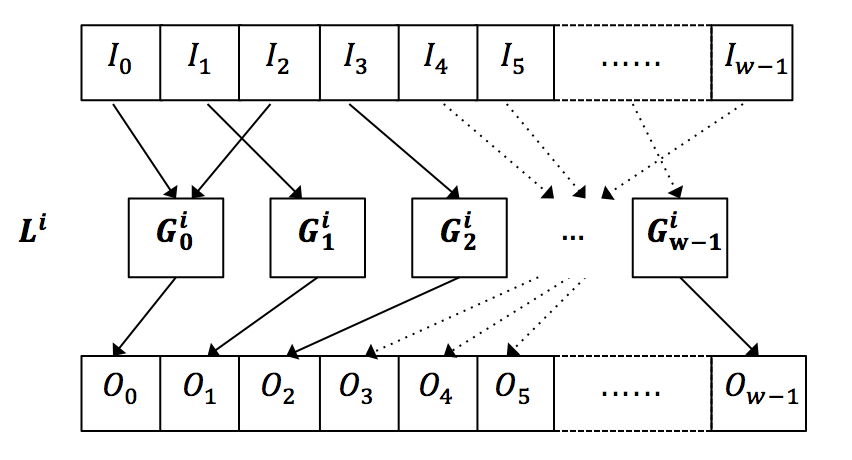
\includegraphics[width=0.8\textwidth]{img/level.png}
	\caption{Simple description of Level $L_i$ evaluation}
	\label{fig:level}
\end{figure}
\par
\subsection{Hardware}
Obfuscators might occasionally run on super computers, however it is likely that viable commercial use of obfuscators would require them to run on mass market platforms such as smart phones, battery powered laptops and desktop computers\cite{clark}. The target platform for the circuits evaluation is a mid-level desktop computer. The CPU is a 64-bits-instruction-set 	 with a base frequency of 3.40 GHz (Max of 4.1GHz). It has 4 cores that can run a thread each and has the following cache capacities (in bytes): 
\begin{itemize}[noitemsep]
\item Level 1 data cache: 32K
\item Level 1 instruction cache: 32K
\item Level 2 cache: 256K
\item Level 3 cache: 6144K
\end{itemize}
We predict that having a circuit with a width higher than the capacity of the last-level cache is a perfect candidate to observe an impact on performance.
\par
The operating system used is Linux Fedora 22 on kernel 4.4.5.


\subsection{Metrics}
The \textit{perf} linux command was used to measure the impact of evaluating a circuit on the CPU. \textit{perf} is a tool written in \text{C} that uses Performance Counters to profile an application\footnote{\url{https://github.com/torvalds/linux/tree/master/tools/perf}}. Performance counters are CPU hardware registers that count hardware events such as instructions executed, cache-misses suffered, or branches mispredicted\cite{perfwiki}. The \textit{perf} tool has the advantage of being program oriented, instead of system oriented \cite{ibm}.   In particular, the \textit{perf stat} subcommand allows to retrieval event counts that are of interest to our experiment. These metrics are mainly \textit{instructions, cycles} and \textit{LLC-loads}. 
\begin{itemize}
\item \textbf{instructions} are unitary operations executed by the CPU at the lowest level such ADD, SUB, LOAD or STORE. They can represent arithmetic operations, data handling operations or control flow operations. Modern CPUs include more complex instructions for complicated integer or float point operations.
\item \textbf{cycles} are the steps performed by the CPU when it recieves an instruction. Typically early processors would pipeline fetching the instruction from the program counter, decoding it, reading its associated variables from the registers, executing its logic order and finally writing the result back to registers or storing it the system's main memory\cite{jmor}. After an initial set up time, pipelining allows to execute one instruction per cycle, assuming no stalls. Modern CPUs achieve more than on instruction per cycle using techniques like \textit{Instruction-level Parallelism} (loading more than one instruction in the pipeline) and \textit{out-of-order execution} (allowing the simultaneous execution of multiple instructions that don't depend on each other for input or output). The Intel Core i5 can handle up to 4 instructions per clock cycle\cite{agner}, but this figure is usually lower because of stalls, i.e.\ when the pipeline is waiting for the result of a previous instruction before proceeding.

\item \textbf{LLC-loads} are instructions to load results from the Last-Level of Cache (or L3) of the CPU. L3 cache is the largest and highest-latency level of cache for the Intel Core i5 CPU. It is shared amongst all its cores.

\end{itemize}
For every value of $w$, we configure \textit{perf} to run the experiment 3 times and collect the arithmetic average of the event counters.


\section{Simulation Results}
In this section we present the results of our experiment.
\par
We suggest that the total running time of a circuit follows the analytical model:
\begin{equation}
T = \max\{ t_g + t_e, t_m(w) \}
\end{equation}
where $T$ is the total elapsed (wallclock) time in processing a single gate, $t_g$ is the CPU time for generating a gate, $t_e$ is the CPU time for evaluating a gate, and $t_m(w)$ are the memory-stalls from the gate-generation and gate-evaluation computations.
\par
In our experiment, we generate the entire circuit prior to its evaluation. $t_g$ is in fact related to the time cost of loading of the gate for execution. We assume that this time component is near constant per gate and is not affected by the width $w$. The generation step executed initially is therefore not monitored for performance. The resulting circuit is stacked gate by gate in a simplified BPW file. Following the initial BPW format developed by Thomborson, the first 4 bytes represent the header of the a BPW file\cite{clark}. The following bytes then represent the total gates of the circuit. All gates are sequentially represented from index $0$ to index $10^8-1$. A given gate's encoding varies from 9 to 25 bytes. The first byte holds the type of the gate. The following 8 to 24 bytes present the input indices encoded over 64-bits each. The gate's representation could be optimised to the minimum bytes needed to encode a gate. Compression could also be used to save disk space. We chose to keep the existing model for simplicity. As mentioned earlier, the size of the circuits under test was fixed to $N = 10^8$. The average size of a BPW file storing a circuit is therefore $avg(sizeof(Gate)) * 10^8 \approx 2 GB$ \footnote{We modelled 14 types of Gates; 1 $\times$ 1-input, 6 $\times$ 2-input and 7 $\times$ 3-input gates. On average, a gate has 2.43 inputs encoded with 8 bytes per input plus one byte for the gate type.}.

\begin{table}[]
\centering
\begin{tabular}{|l|l|l|l|}
\hline
w                 & $10^3$       & $10^4$       & $10^5$       \\ \hline
task-clock (ms)   & 13116.554712 & 13322.905953 & 13313.335011 \\ \hline
instructions      & 99200423097  & 97602445259  & 97553743526  \\ \hline
cycles            & 55393862507  & 56255744084  & 56207517444  \\ \hline
instruction/cycle & 1.74         & 1.76         & 1.74         \\ \hline
branches          & 17179168771  & 16896966649  & 16887492840  \\ \hline
branch-misses     & 213275235    & 267635214    & 267596585    \\ \hline
LLC-loads         & 75319029     & 75177952     & 78311853     \\ \hline
std deviation     & 1.49\%       & 0.94\%       & 0.27\%       \\ \hline
\end{tabular}
\caption{Simulation results for $ w \in \{10^3, 10^4, 10^5\}$ }
\label{tab:res1}
\end{table}


\begin{table}[h]
\centering
\begin{tabular}{|l|l|l|l|}
\hline
w                 & $10^6$      & $10^7$      & $10^8$       \\ \hline
task-clock (ms)   & 13633.97763 & 16041.15891 & 17507.07431  \\ \hline
instructions      & 97578653791 & 98201779911 & 103646369628 \\ \hline
cycles            & 57584456723 & 67736311966 & 73941409511  \\ \hline
instruction/cycle & 1.69        & 1.44        & 1.4          \\ \hline
branches          & 16897296695 & 17058902603 & 18501020880  \\ \hline
branch-misses     & 266970610   & 266910904   & 268274635    \\ \hline
LLC-loads         & 328139283   & 380853849   & 505923626    \\ \hline
std deviation     & 0.43\%      & 0.50\%      & 0.19\%       \\ \hline
\end{tabular}%
\caption{Simulation results for $ w \in \{10^6, 10^7, 10^8\}$}
\label{tab:res2}
\end{table}


\par
From the results collected in tables \ref{tab:res1} and \ref{tab:res2} we established the following:

\[ T =
  \begin{cases}
    t_g + t_e       & \quad \text{if } \log_{10}(w) < 7\\
    t_m(w) & \quad \text{if } \log_{10}(w) > 7\\
  \end{cases}
\]

We estimate that $t_m(w)$ for $w = 10^3$ is negligible. In our experiment $E(w = 10^6)$ the total run time is assumed to reflect load and execution operations only (with no width penalty) which establishes $t_g + t_e \approx 130\text{ ns}$.\footnote{ For $w = 10^3, N=10^8$, we have $N \times T = 13116 \text{ms} \implies T \approx 130 \text{ns}$ }. 
Since the CPU has a frequency of 3.40 GHz the load and execution of a gate require about 450 CPU cycles per gate\footnote{$130 \times 10^{-9} \times 3.4 \times 10^9 = 442$}, which is up to 2000 instruction per cycle (at 1.7 instructions per cycle) on a quad-core CPU assuming no stalls. For all tested $w < 10^7$ we observed a stable instruction per cycle rate at 1.7 ins/cycle with 0.2 instruction per cycle stalled.
\par
For $ w > 10^7$ the computation becomes memory-bound, allowing us to estimate $t_m(10^7) = 162$ns and $t_m(10^8) = 176$ns. Since we used 6 types of 2-input gate and 7 types of 3-input gate (out of a total 14 gate types), a gate evaluation will have 1 fetch to read the gate type and about 2.5 memory-fetches on average to read its inputs. The gate evaluation process will also write the result in the output buffer which will cause additional memory writes. 
\par
Once the gate is unpacked in a top-level \textit{C} \textbf{struc} of 16 bytes (1 byte for the type, 8 bytes for the input pointer, before padding to the largest power of 2), with 2.5 input indices of 8 bytes each, a level needs $ (16 + 2.5 \times 8) \times w $ of memory to be fully represented, e.g.\ levels for $w = 10^7$ need 3.6 GB. This amount of memory cannot obviously reside in cache, and on 4 GB memory platforms there would certainly be page-faults requiring hard disk activity. We estimate that the level array can fit inside our system's 16GB RAM without disk faults. Our initial algorithm loads an entire level before feeding into the execution loop. We could improve this by evaluating a gate as soon as it is loaded.  
\par
We designed the gate inputs to be spread randomly in an array of width $w$. For any large enough $w$, the CPU last level cache (LLC) will miss with a high probability when the input bit-array cannot be fully contained. On our test platform, LLC is 6MB wide and the cache line is 64B\cite{agnor}. 
\par
For $w = 10^7$, the input array occupies $8 \times 10^7$ bits, the miss rate should be $1 - (6\times10^6B/10^7B) = 40\%$. From the observed $T = 162ns$ we deduce the memory latency, which is the time required by the CPU to fetch a gate input from the cache, to be $162ns$ per LLC miss.\footnote{ $latency = \frac{T}{2.5 \times \text{miss rate}}$ where $T$ is the total run time per gate}. Each unpacked level occupies $ 36\times10^7$ bytes in memory. For the observed run time this is equivalent to 225 MB/s in memory bandwidth. The reported LLC-loads represent about 10\% for the bandwidth at 23.5 MB/s. However, the cache line being 64B wide, the LLC-loads represent 1.3 GB/s bandwidth. With the estimated latency, there should be a a gate input miss every 162ns. This gives us a bandwidth of 453 MB. We suspect that the 900 MB difference noted is possibly due to the read and write traffic caused by the writing of the results back into the output array.
\par
The Ivy Bridge CPU family, to which our test CPU belongs, also seems to have a problem with the pre-fetch instructions wasting time on pre-fetching data that are already in the cache\cite{agnor} which might explain the high bandwidth observed.
\par
Based on the data on this paper, we could not observe significant hit on the overall performance when evaluating wide circuits. This might be explained by the CPU's successful speculative optimisation of branch mispredictions. We also suspect that the generation of random 64-bit input indices using the C \textit{rand()} method (which returns a random 32-bit integer) might produce numbers with the most significant bits 75\% biased towards 1\footnote{\url{http://stackoverflow.com/questions/4945698/is-the-value-of-rand-max-always-2n-1}}
. This will affect the memory-fetch statistics for gates with large indices.



\section{Discussion and Future Work}
Obfuscation is a potentially powerful tool to encrypt and protect data in the
future. However, one of the limitations of obfuscation may prove to be that it
lowers the execution speed of a programme, at least in some circumstances.
\par
In this experiment we simulated an obfuscated circuit by generating a fixed-width
random boolean circuit and evaluated the performance of that circuit. We have
shown how \textit{perf} hardware counters can be used to measure cache hits
inside a 6MB L3-cache ix86 microprocessor clocked at 4GHz in order to evaluate
a simulated obfuscated circuit.
\par
We have proposed an analytical model to explain the execution times observed. Data
collected for width $w > 10^6$ falls outside the confidence interval of the regression
curve of smaller widths. Further statistical analysis will be done before this work
will be published in a technical journal. In this study our assumption was that when $w$ is large, it would be
possible to seperate $t_g + t_e$ and $t_m$, as $t_g + t_e$ would become negligible as $t_m(w)$ would increase
significantly and dominate the results. However the results obtained failed to
match this prediction
\par
In future work, we plan to optimise the code so that a gate evaluation would be
performed in tens of CPU cycles only. Although our CPU has a maximum specification of 8 instructions per cycle\ref{}, we think
that attaining that ceiling will be quite hard since most of those instructions are
low-level instructions needed internally by the CPU.
\par
We hope however that by reducing $t_e$ by a factor 10 we can better evaluate
$t_m(w)$ and $t_g$. Our current experiment was not optimised for $t_g$ or $t_m(w)$.
By generating the entire circuit prior to evaluation, the computation was either memory bound,
file-IO bound, or stalls and cache-conflict bound when the output of the generator process
was piped to the input of the evaluator process. We can also improve the size of program in memory by encoding input and output values over
1 bit rather than the current 1 byte encoding.
We believe that there is a trade off between memory and CPU when evaluating $t_g$.
When not reading from a file descriptors, gates would be created using random number generators
that would require extra CPU cycles.
\par
We don't think that designing a multithreaded experiment
will improve the observed running speed if the memory bandwidth of the
CPU is already saturated and that $t_(w)$ can only be lowered by reducing the memory loads to a minimum.
\par
We are also focusing on improving our simulation by replacing the random generation
mechanism using the \textit{C} standard library \textit{rand()} method with the
’stride’ approach\cite{stride} to remove any bias in generating large random
integers and break any predictability patterns.
\par
Future work would explore the use of the Intel Performance Counter Monitor
library\footnote{\url{https://software.intel.com/en-us/articles/intel-performance-counter-monitor}}
as a high level interface for measuring real time performance data directly
inside the circuit's code to separate . In particular, we plan to measure the
CPU cache and instruction metrics at initialisation time, then at generation
time and finally at execution time to isolate each stage's impact on performance.
\par
A more extensive study, using a large range of hardware devices and over
a large range of circuit simulations, could also help validate or disprove the
proposed model.

%-----------------------------------------------------------
\printbibliography
%-----------------------------------------------------------
\end{document}
